\chapter{Einleitung}

    Dieser Projektbericht ist im Rahmen der Cross Innovation Class 2022 entstanden.

\section{Cross Innovation Class}

    Die Cross Innovation Class, kurz CIC, ist eine von der Hamburg Kreativ Gesellschaft organisierte Veranstaltung in Kooperation mit Universitäten und Fachhochschulen des Hamburger Umlands.
    Idee der CIC ist es Studierende verschiedener Fachrichtungen unterschiedlicher Universitäten ein Semester lang in interdisziplinären Teams an Projekten zusammenarbeiten.

    Teilnehmen konnten Studierende des Studiengangs Stadtplanung der Hafencity Universität Hamburg, der Studiengänge Produkt- und Interior-Designer der Akademie Mode \& Design des Standorts Hamburg und der Studiengänge Informatik, Technische Informatik, Wirtschaftsinformatik, Smart Technology und IT-Ingenieurwesen der Fachhochschule Wedel.

    Die Cross Innovation Class lief dabei dieses Jahr unter dem Thema Resilient Cities. In Bezug auf dieses Oberthema wurden fünf Partnerunternehmen ausgesucht, die jeweils eine Fragestellung mit in die CIC gebracht haben.


    \vspace{1em}
    \framebox[\textwidth]{
        \begin{minipage}{\textwidth-1em}
            \vspace{.4em}
            \textbf{Resilient Cities}
            \\ \\
            Resilienz, ein wichtiger Faktor in vielen Lebensbereichen.
            Ein Attribut das Anpassungsfähigkeit und einen standhaften Umgang mit Krisen beschreibt.
            Neben persönlicher und ökonomischer Resilienz übernimmt Resilienz auch eine immer wichtiger werdende Rolle im Blick auf Gemeinden und Städte.
            Vorallem im Bezug auf Extremwetterereignisse und dem immer weiter voranschreitenden Klimawandel braucht es neue Ideen und Konzepte.
            \\ \\
            Daher gibt es viele Bestrebungen auf globaler, europäischer und nationaler Ebene dieses Thema voranzubringen. Eine Institution ist der Urban Resilience Club, der Urbane Resilienz wie folgt definiert:
            \\
            \enquote{Urban Resilience - The measurable ability of any urban system, with its inhabitants, to maintain continuity through all shocks and stresses, while positively adapting and transforming toward sustainability.}\footnote{\url{https://urbanresiliencehub.org/what-is-urban-resilience/}}
            \\
        \end{minipage}
    }
    \vspace{1em}
    
    Partner dieses Jahr waren die Stadt Frankfurt mit der Stabsstelle Digitalisierung, die ACO Gruppe, Hamburg Marketing, Hamburg Institute for Innovation, Climate Protection and Circular Economy (HiiCCE) und das Wald Stadt Labor Iserlohn. \\

    Fünf Teams, jeweils bestehend aus Studierenden jeder Universität und einem Praxispartner durchliefen über knapp 12 Wochen ein Ablauf im Rahmen des Design Thinkings.

    Dieses Format stellt im Vergleich zu den sonst eher theoretischeren oder fachspezifischeren Veranstaltungen eine willkommene Ergänzung da.

    \subsection{Ablauf der CIC}

        Das Projekt wurde in drei große Phasen eingeteilt, Konzept, Entwurf und Prototyping.

        Neben einem KickOff zu Beginn gab es am Ende jeder Phase eine Feedback Runde mit der gesamten Class.
        
        In der KickOff Veranstaltung haben sich die Praxispartner und ihre Fragestellung vorgestellt und wir haben unser Team kennengelernt.

        Zusätzlich wurde allen Interessierten vor der Abschlussveranstaltung ein sehr lehrreiches Pitch-Training angeboten.

        Wie sind die Teams enstanden, was hatten wir für (Regel)Termine, wie viel Zeit hatten wir für die unterschiedlichen Aufgaben, etc.
        Skizzierung des CiC-Prozesse.

    \subsubsection{Projektphasen}

        \begin{center}
            \begin{tabular}{ |l|l| }
                \hline
                Termin/Phase & Bezeichnung \\
                \hline
                \hline
                \printdate{2022-04-08} & Kick-Off \\
                \hline
                \printdate{2022-04-11} - \printdate{2022-04-21} & Analyse \& Konzept Phase \\ 
                \hline
                \printdate{2022-04-25} - \printdate{2022-05-06} & Entwurfsphase \\
                \hline
                \printdate{2022-05-09} - \printdate{2022-06-23} & Prototyping \& Modellbau Phase \\
                \hline                
                \printdate{2022-06-30} & Abschlussveranstaltung \\
                \hline
            \end{tabular}
        \end{center}


    \subsubsection{FH Wedel JourFixe}
        
        Analog zur AMD und HCU hatten wir ein wöchentliches internes Meeting an der FH Wedel.
        Ziel dieses Meetings war ein Statusbericht der jeweiligen 


    \subsubsection{Gruppen \& Praxispartner JourFixe}
        
        Zusätzlich haben wir uns intern jeden Donnerstag um 8:30 Uhr getroffen um offene Fragen und anstehende Aufgaben zu besprechen.
        Um 10 Uhr kamen daraufhin unsere Praxispartner dazu, sodass wir aufgekommene Fragen klären konnten und einen Bericht über den aktuellen Stand un die anstehende Woche geben konnten.



\section{Das Team}

        Unser Team bestand aus sieben Studierenden. Drei Studierenden der Hafencity Universität des Studiengangs Stadtplanung, Celina Krug, Moritz Hillen und Florian Bucher, zwei Studierende der Akademie Mode \& Design des Studiengangs Product Design und uns, Sven Hülsen und Robin von Berg, Informatikstudenten der FH Wedel.

        Aus der AMD unterstützt wurden wir ebenfalls von Annika Fröhlich, da dort eine weitere interne Unterteilung in Gruppen angesetzte wurde, die gemeinsam mehrere Projekte (eins davon die CIC) bestritten haben.

        \begin{figure}[h]
            \begin{center}
                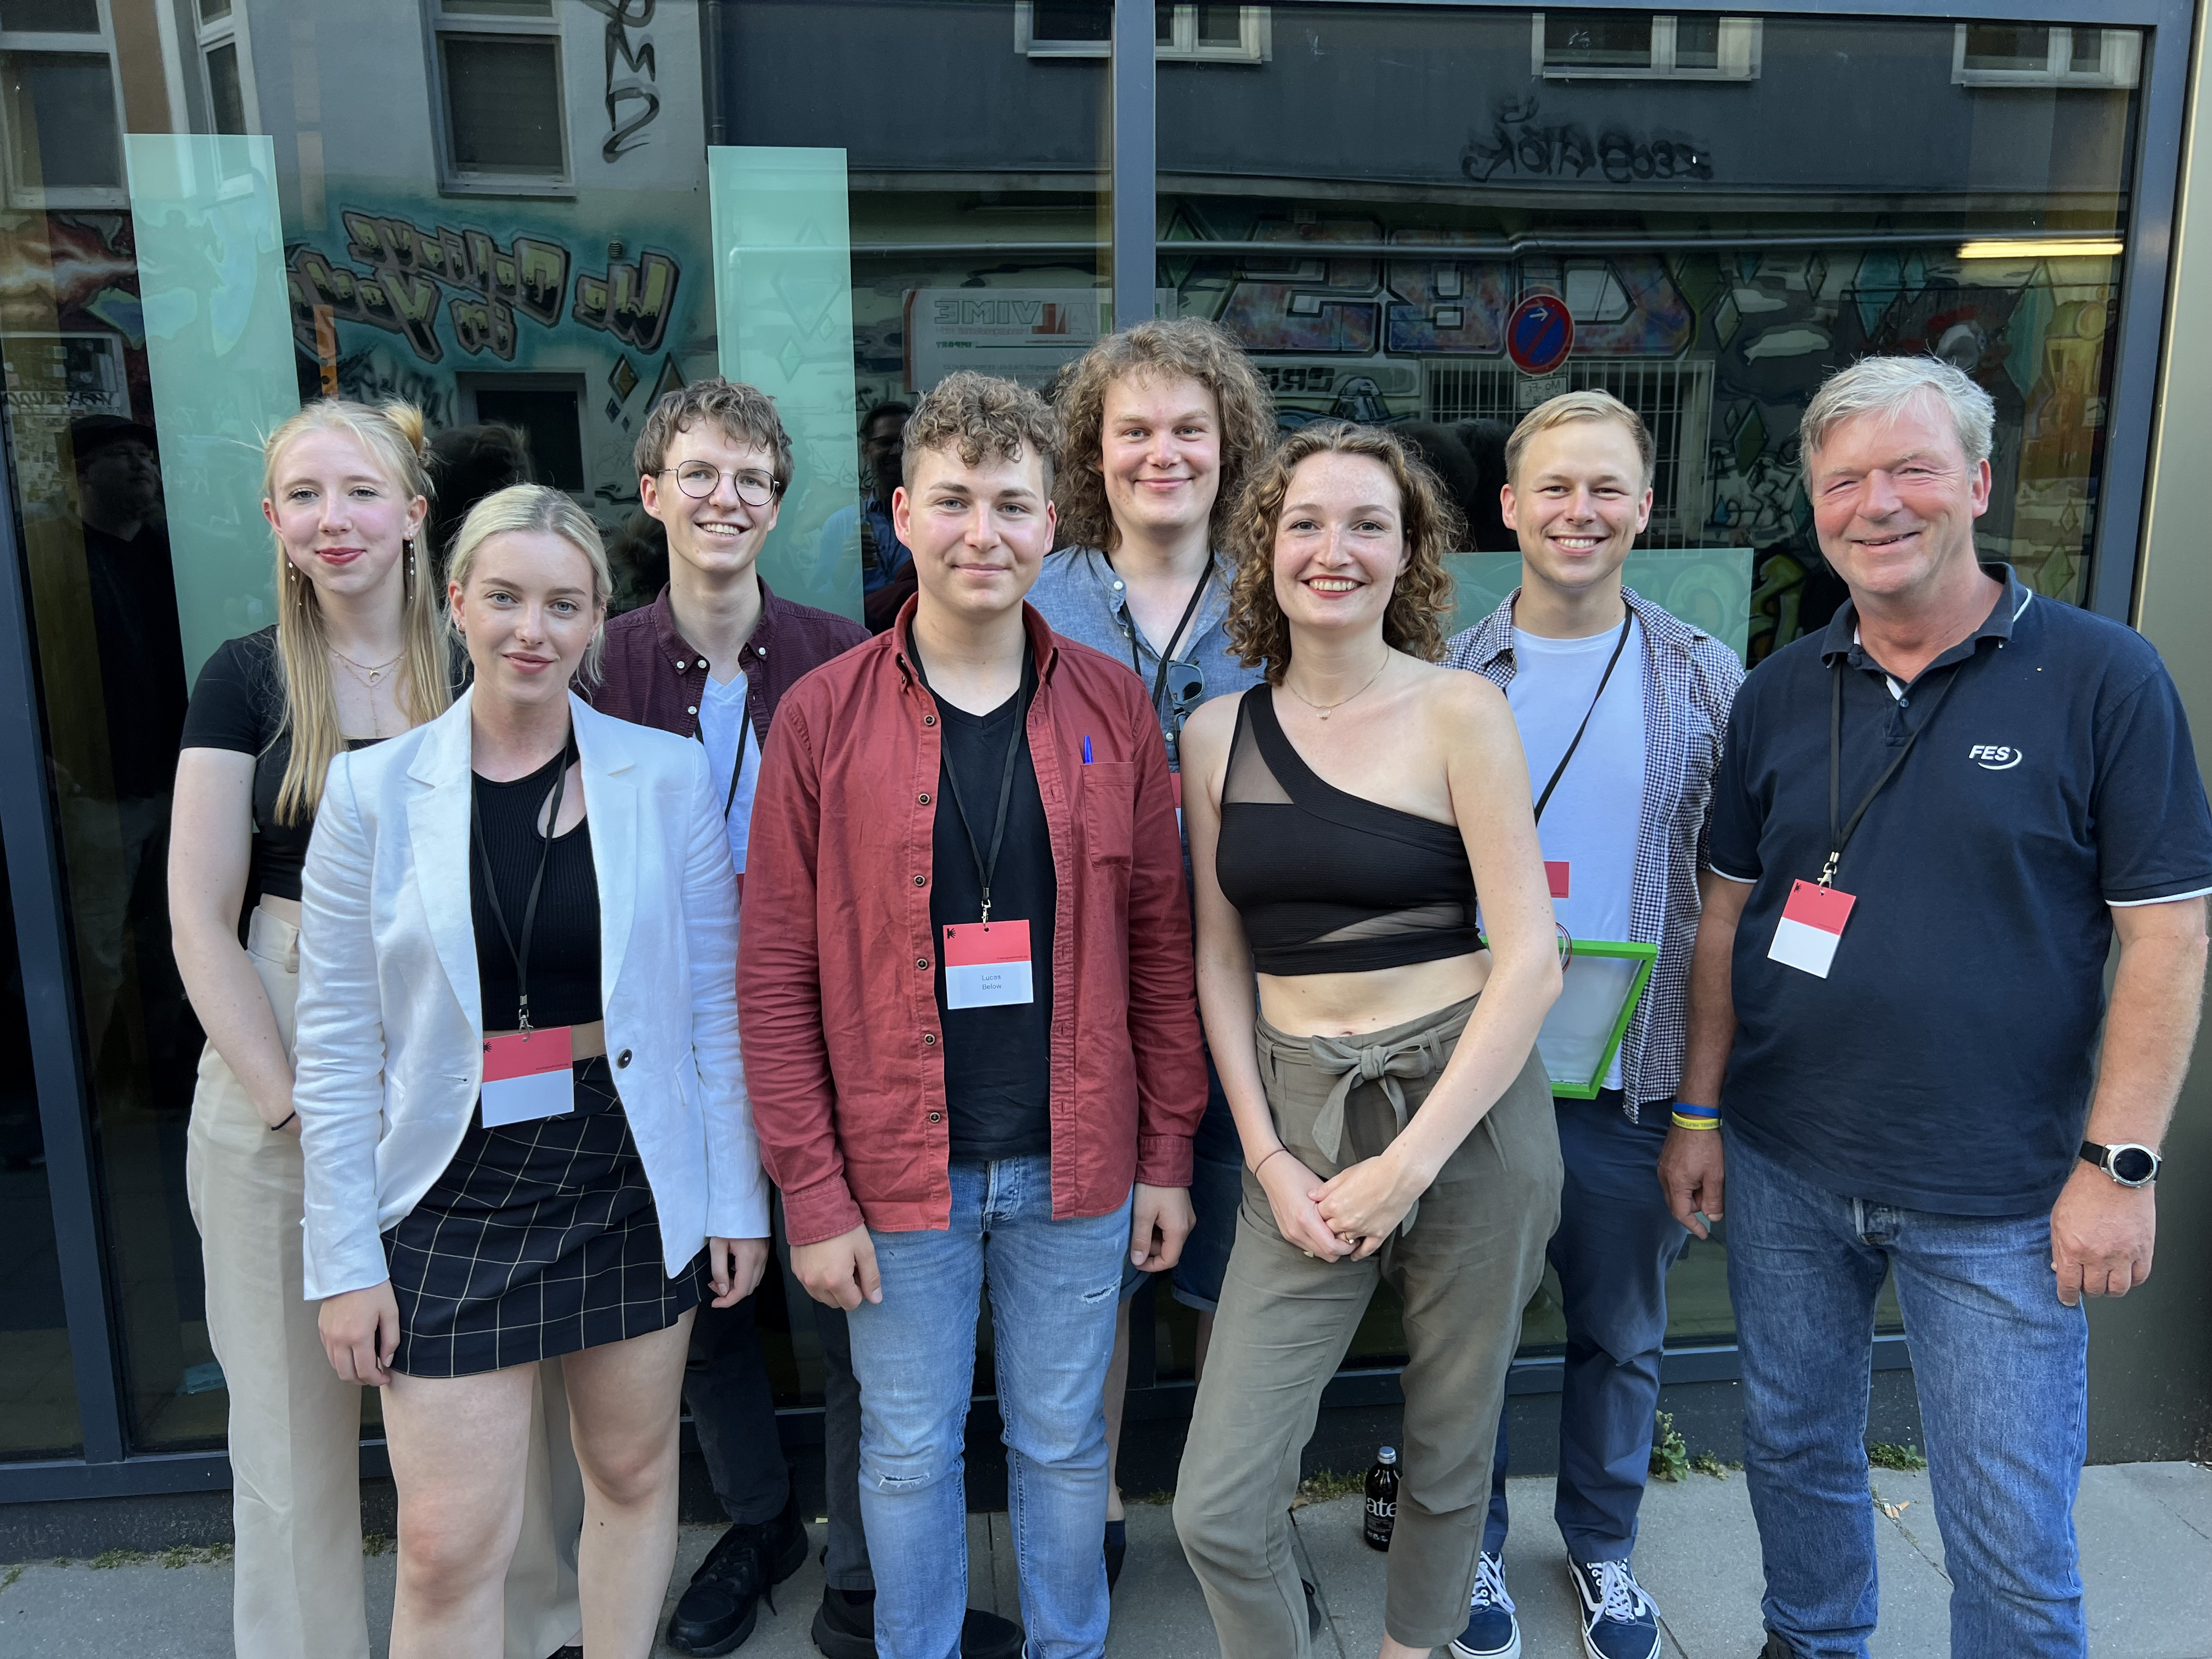
\includegraphics[width=11cm]{media/00_introduction/pic_team-FFM.jpg}
            \end{center}
            \caption[CIC Team Stadt Frankfurt]{CIC Team Stadt Frankfurt \par \small v.l.n.r.: Maybritt Braun (AMD), Annika Fröhlich (AMD), Robin von Berg (FHW), Lucas Below (AMD), Sven Hülsen (FHW), Celina Krug (HCU), Moritz Hillen (HCU), Jochen Schmitz (FES). Abwesend: Florian Bucher (HCU), Mechthild Schulze-Tenberge \& Karina Mombauer             (Stadt Frankfurt Stabstelle Digitalisierung)}
            \label{fig:team_frankfurt}
        \end{figure}

\section{Unsere Praxispartner}
    Zu Beginn der CIC hat Mechthild Schulze-Tenberge als Ansprechpartnerin der Stadt Frankfurt am Main agiert.
    Frau Schulze-Tenberge übernimmt die Leitung der Stabstelle Digitalisierung und war diejenige, die uns die Aufgabenstellungen der Stadt Frankfurt präsentiert hat.

    Im späteren Verlauf hat Karina Mombauer, ebenfalls aus der Stabstelle Digitalisierung, ihren Platz übernommen, da Frau Schulze-Tenberge andere Projekte verfolgen musste. \\

    Als Unterstützung und Experte zum Thema Stadtreinigung ist Jochen Schmitz zum Projekt hinzugestoßen. Als Leiter des Innovationsmanagement der FES konnte er uns Einblicke in die alltäglichen Abläufe und Erfahrungen der FES, der internen Projekte bezüglich Sensorik und Kommunikationsansätzen geben, aber zusätzlich auch eine weitere Perspektive auf die vorhandenen IT-Projekte der Stadt Frankfurt. \\

    Zusätzlich wurden wir von Dagmar Schöne unterstützt, die Teil des Teams \enquote{\#cleanFFM} war und somit die andere Seite, die Rolle der Auftraggeberin der FES übernommen hat.
    
    \subsection{Stadt Frankfurt am Main - Stabstelle Digitalisierung}

        Die Stabstelle Digitalisierung der Stadt Frankfurt am Main existiert seit 2021 und ist der Nachfolger der im Jahre 2013 gegründeten Stabstelle E-Government, die als Ziel die möglichst durchgehend elektronische Abwicklung von Verwaltungsvorgängen hatte.
        
        Bei der Umstrukturierung zur Stabstelle Digitalisierung sind weitere Themen zum Aufgabengebiet hinzugekommen.
        In diesem Zuge wurde eine \enquote{Gesamtstädtische Digitalisierungsstrategie} (\href{run:attachments/Frankfurt_Digitalisierungsstrategie.pdf}{\textbf{PDF}}) entwickelt.
        Diese umfasst unter anderem eine \enquote{Urban Data Plattform} und den flächenüberdeckenden Ausbau eines LoRaWAN Netzes.


    \subsection{Frankfurter Entsorgungs- und Service GmbH (FES)}

        Die Frankfurter Entsorgungs- und Service GmbH, kurz FES, ist das Frankfurter Äquivalent zur Stadtreinigung Hamburg. 
        Das seit 1995 bestehende Unternehmen beschäftigt circa 1900 Mitarbeiter und bietet neben Entsorgungs- und Reinigungsdienstleistungen bspw. auch Verkehrsmaßnahmen und ein Veranstaltungsservice an.
        Desweiteren hält die FES 50 Prozent der FFR GmbH, die das Müllheizkraftwerk Frankfurt am Main betreibt.
